\iffalse
\let\negmedspace\undefined
\let\negthickspace\undefined
\documentclass[journal,12pt,twocolumn]{IEEEtran}
\usepackage{cite}
\usepackage{amsmath,amssymb,amsfonts,amsthm}
\usepackage{algorithmic}
\usepackage{graphicx}
\usepackage{textcomp}
\usepackage{xcolor}
\usepackage{txfonts}
\usepackage{listings}
\usepackage{enumitem}
\usepackage{mathtools}
\usepackage{gensymb}
\usepackage{comment}
\usepackage[breaklinks=true]{hyperref}
\usepackage{tkz-euclide} 
\usepackage{listings}
\usepackage{gvv}                                        
\def\inputGnumericTable{}                                
\usepackage[latin1]{inputenc}                            
\usepackage{color}                                       
\usepackage{array}                                       
\usepackage{longtable}                                   
\usepackage{calc}                              
\usepackage{tikz}
\usepackage{multirow}                                    
\usepackage{hhline}                                      
\usepackage{ifthen}                            
\usepackage{caption}
\usepackage{lscape}
\usepackage{amsmath}
\newtheorem{theorem}{Theorem}[section]
\newtheorem{problem}{Problem}
\newtheorem{proposition}{Proposition}[section]
\newtheorem{lemma}{Lemma}[section]
\newtheorem{corollary}[theorem]{Corollary}
\newtheorem{example}{Example}[section]
\newtheorem{definition}[problem]{Definition}
\newcommand{\BEQA}{\begin{eqnarray}}
\newcommand{\EEQA}{\end{eqnarray}}
\newcommand{\define}{\stackrel{\triangle}{=}}
\theoremstyle{remark}
\newtheorem{rem}{Remark}

\begin{document}

\bibliographystyle{IEEEtran}
\vspace{3cm}

\title{NCERT Math 11.9.2 Q8}
\author{EE23BTECH11009 - AROSHISH PRADHAN$^{*}$% <-this % stops a space
}
\maketitle
\newpage
\bigskip
\textbf{Question:} If the sum of $n$ terms of an AP is $(pn + qn^2)$, where $p$ and $q$ are constants, find the common difference.

\solution
\fi
\begin{table}[!h]
    \centering
    \begin{tabular}{|c|c|c|}
    \hline
      \textbf{Symbol}   &  \textbf{Value} & \textbf{Description}\\
    \hline
       $y(n)$  & $(pn + qn^2)$ & Sum of $n$ terms\\
    \hline
        $x(n)$ &  & $n^{th}$ term of AP\\
    \hline
        $d$ & $x(n+1) - x(n)$ &Common Difference\\
    \hline 
\end{tabular}

    \caption{Given Parameters}
    \label{tab:1}
\end{table}

Sum of $n$ terms, as a discrete signal:
\begin{align}
    y(n) = (pn + qn^2)u(n) \label{eq:1}
\end{align}
Taking the $Z$-Transform,
\begin{enumerate}
    \item $\mathcal{Z}\{u(n)\}$
\begin{align}
    u(n) \system{Z} \frac{1}{1-z^{-1}} \{\abs{z} > 1\} \label{eq:2}
\end{align}
    \item $\mathcal{Z}\{nu(n)\}$
\begin{align}
    nu(n) \system{Z} \frac{z^{-1}}{(1-z^{-1})^2}\, \{\abs{z} > 1\} \label{eq:3}
\end{align}
\item $\mathcal{Z}{\{n^2 u(n)\}}$
    \begin{align}
        n^2u(n) \system{Z} \frac{z^{-1}(1+z^{-1})}{(1-z^{-1})^3}\, \{\abs{z} > 1\} \label{eq:4}
    \end{align}
\end{enumerate}
Taking the Z-Transform of \eqref{eq:1} using \eqref{eq:3} and \eqref{eq:4}
\begin{align}
      Y(z) = p\brak{\frac{z^{-1}}{(1-z^{-1})^2}} + q\brak{\frac{z^{-1}(1 + z^{-1})}{(1-z^{-1})^3}}
\end{align}
Now, 
\begin{align}
    y(n) &= x(n) \ast u(n)\\
    \implies Y(z) &= X(z)U(z)\\
    \implies X(z) &= \frac{Y(z)}{U(z)}\label{eq:8}
\end{align}
Using \eqref{eq:2} in \eqref{eq:8},
\begin{align}
    X(z) &= p\brak{\frac{z^{-1}}{(1-z^{-1})}} + q\brak{\frac{z^{-1}(1 + z^{-1})}{(1-z^{-1})^2}}
\end{align}
Using contour integration for inverse Z-Transform:
\begin{align}
    x(n) &= \frac{1}{2\pi j} \oint_C X(z) z^{n-1}dz\\
    &= \frac{1}{2 \pi j} \oint_C  \sbrak{p\brak{\frac{z^{-1}}{(1-z^{-1})}} + q\brak{\frac{z^{-1}(1 + z^{-1})}{(1-z^{-1})^2}}}z^{n-1}dz
\end{align}
Calculating the residues $R_1$ and $R_2$ at pole $z=1$:
\begin{align}
    R_1 &= \frac{1}{0!} \lim_{z \to 1}(z-1)\brak{p\brak{\frac{z^{-1}}{1-z^{-1}}}}z^{n-1}\\
    &= p\\
    R_2 &= \frac{1}{1!} \lim_{z \to 1}\frac{d}{dz}\brak{(z-1)^2q\brak{\frac{z^{-1}(1 + z^{-1})}{(1-z^{-1})^2}}}z^{n-1}\\
    &= q\lim_{z \to 1}\frac{d}{dz}\brak{z^{n} + z^{n-1}}\\
    &= q(2n-1)\\
    \implies x(n) &= R_1 + R_2\\
    &= p + q(2n-1)
\end{align}
Writing x(n) as a discrete signal we get:
\begin{align}
    x(n) &= (p-q)u(n) + 2qnu(n)\label{eq:19}
\end{align}
To simplify, use $n=0$:
\begin{align}
    y(0)&=x(0)\\
    \implies 0 &= (p-q)u(0) +2q(0)u(0)\\
    \implies p &= q
\end{align}
$\therefore$ \eqref{eq:19} an be written as:
\begin{align}
    x(n) &= 2qnu(n)
\end{align}
Common difference is given by:
\begin{align}
    d &= x(n+1) - x(n)\\
    &= 2q
\end{align}
\begin{figure}[!h]
    \centering
    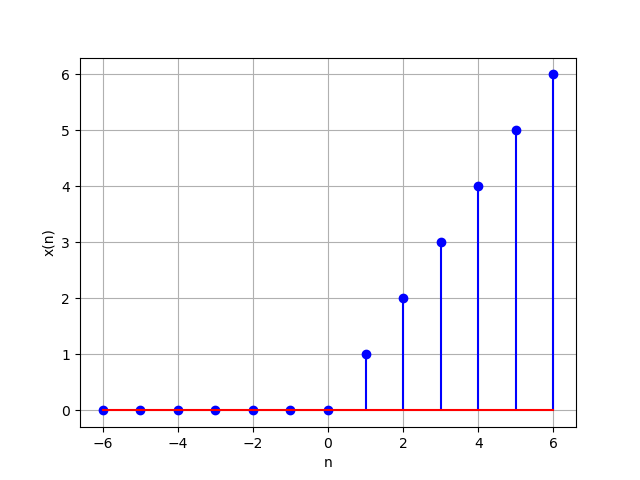
\includegraphics[width = \columnwidth]{ncert-maths/11/9/2/8/figs/x_plot.png}
    \caption{Plot of x(n) vs n for $p=q=0.5$}
    \label{fig:1}
\end{figure}
\begin{figure}[!h]
    \centering
    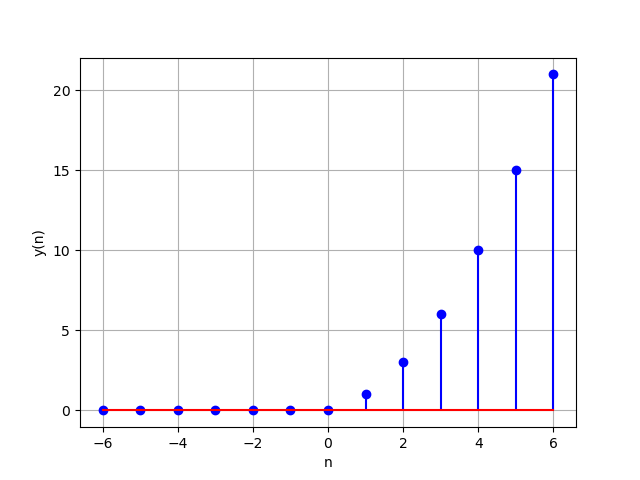
\includegraphics[width = \columnwidth]{ncert-maths/11/9/2/8/figs/y_plot.png}
    \caption{Plot of y(n) vs n for $p=q=0.5$}
    \label{fig:2}
\end{figure}
